\subsection{Backend}
Das Backend besteht aus mehrere Paketen und ist wie folgt aufgebaut:
\begin{figure}[H]
	\centering
	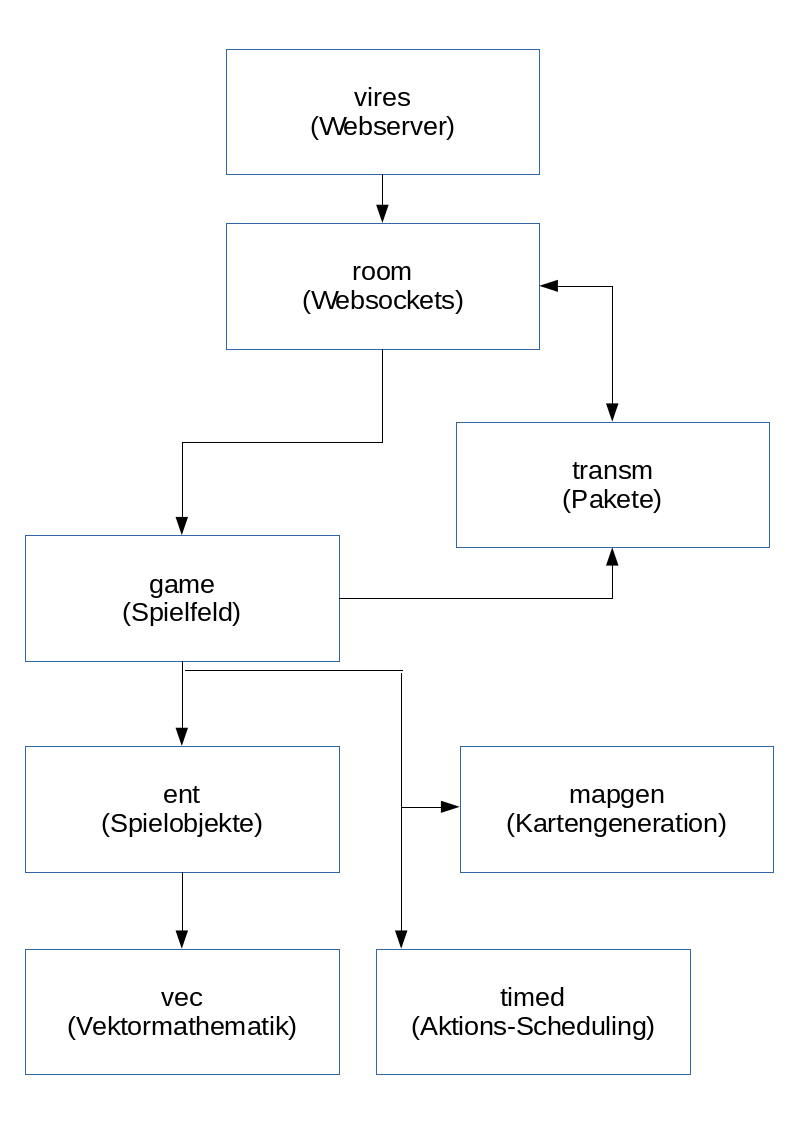
\includegraphics[width=0.8\textwidth]{Architektur.png}
\end{figure}
Die Bedeutung der einzelnen Pakete und wichtige Algorithmen werden im Folgenden erklärt.

\subsubsection{vires}
\verb+vires+ ist das Main-Package des Programms und kümmert sich um die Verwaltung des Webservers von \vires. \\
Wird eine GET-Anfrage auf einen Link ausgeführt, der eine Room-ID enthält (z.B. \url{http://localhost/1234}), so wird eine Template für den Raum, welche mit der Room-ID kompiliert wird, an den User gesendet. \\
Die kompilierte Template öffnet hieraufhin eine Websocket-Verbindung zu \verb+/<roomid>/c+. \\
Der Handler für \verb+/<roomid>/c+ eröffnet dann auch serverseitig die Websocket-Verbindung und übergibt die Verbindung an die jeweilige \verb+room+-Instanz.

\subsubsection{room}
\verb+room+ verwaltet die Websocket-Verbindungen eines Rooms. Verbindet sich der erste User mit dem Room, so wird der Room erstellt. \\
Alle Operationen eines Rooms werden von einer Monitor-Goroutine verwaltet, welche den Zugriff auf alle Zustände des Rooms synchronisiert. \\
Insgesamt verwaltet die Monitor-Goroutine Spielerverbindungen, Matches, Pakete von und an Nutzer und Pakete vom Spiel. \\
Wird eine Websocket-Verbindung zu dem Room hinzugefügt, so werden für diese Verbindung eine Reader- und eine Writer-Goroutine gestartet. 

\subsubsection{game}
\verb+game+ verwaltet eine Spielinstanz. Eine Spielinstanz wird als Spielfeld ausgedrückt, welches sich um alle Spieloperationen kümmert, welche das gesamte Spielfeld erfordern. \\
Der \vires-Server verfolgt einen anderen Ansatz als die meisten Serverapplikationen von Spielen: 
Anstatt innerhalb eines Game-Loops zu überprüfen, ob bestimmte Bedingungen erfüllt sind,
werden alle Aktionen vorberechnet und mittels Timern und einem Scheduler verzögert, bis die Aktion ausgeführt werden soll. \\
\begin{figure}[H]
	\centering
	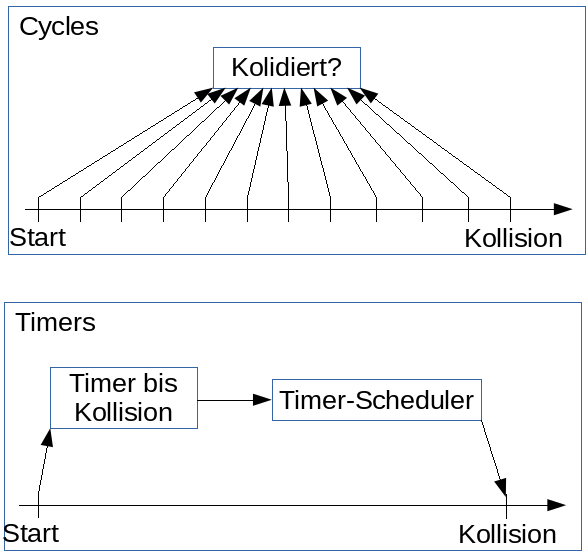
\includegraphics[width=0.8\textwidth]{Timers.png}
\end{figure}
\vires\ ist langsam und der Server soll in der Lage sein, sehr viele Matches gleichzeitig auszuführen. 
Würde der Server für jedes Match Game-Loops verwenden, so wäre entweder die Bearbeitungszeit sehr schlecht oder eine hohe
Überprüfungsfrequenz würde Serverleistung verschwenden. \\
\verb+room+ kommuniziert mit \verb+game+, indem es Methoden von \verb+game+ aufruft, wenn Nutzereingaben erfolgen. \\
\verb+game+ kommuniziert mit \verb+room+, indem es Nachrichten über \verb+transm+ nach \verb+room+ schickt, wenn das Spiel den Spielern etwas mitteilen muss. \\
Insgesamt verwaltet \verb+game+ Movements, Collisions und Conflicts. Jede Aktion auf dem Spielfeld wird über den \verb+timed+-Scheduler
ausgeführt, um Zustandszugriffe vom Spiel und von Nutzern zu synchronisieren. \\
Wird ein Movement gestartet, so wird zuerst geprüft, ob das Movement erlaubt ist. Ist es erlaubt, so wird ein Movement erzeugt, 
ein Conflict am Zeitpunkt des Conflicts für die Target-Cell geschedulet und mit jedem anderen Movement geprüft, ob es eine Collision gibt. \\
Gibt es eine Collision, so wird die Collision beiden kollidierenden Movements hinzugefügt und für den Zeitpunkt der Collision geschedulet.
Tritt der Conflict auf, so wird das Movement entfernt, die Anzahl an Moving Vires je nach Art des Conflicts der Cell hinzugefügt oder der Cell abgezogen,
überprüft, ob die Cell den Besitzer gewechselt hat, überprüft, ob der Besitzer tot ist und geprüft, ob ein Spieler das Match gewonnen hat. \\
Tritt eine Collision auf, so kämpfen die Movements miteinander oder vereinen sich je nach Art der Collision.
Hieraufhin werden alle Collisions beider Movements entfernt und neu berechnet, da die Anzahl an Moving Vires die Größe und die Geschwindigkeit beeinflusst und sich somit auch die Situation für zukünftige Collisions ändert.
Stirbt eines der Movements, so wird der Conflict für das jeweilige Movement entfernt. \\
Es wird also insgesamt beim Erzeugen eines Movements berechnet, welche Collisions nach der aktuellen Situation auftreten können, 
verändert sich aber die Situation auf dem Spielfeld, so werden erst zum Zeitpunkt der Situationsveränderung die jeweiligen Änderungen 
an den anliegenden Movements vorgenommen. \\
Beim Erzeugen der Movements wird zuerst nur davon ausgegangen, dass die auftretenden Collisions alle mit der Startgröße und der Startgeschwindigkeit stattfinden. \\
Hieraus ergibt sich, dass lediglich die anliegenden Movements verändert werden müssen, und nicht rekursiv alle Movements die nach der aktuellen Collision stattfinden. \\
Das folgende Szenario ist anzunehmen:
\begin{figure}[H]
	\centering
	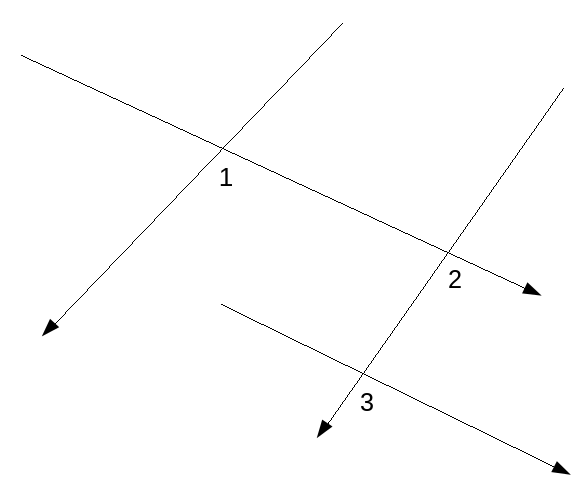
\includegraphics[width=0.8\textwidth]{Collision.png}
\end{figure}
Movements werden als Pfeile dargestellt. Alle vier Movements werden zeitnah hinzugefügt. Beim Hinzufügen aller Movements wird bestimmt, dass mit der Startgeschwindigkeit und dem Startradius des Movements die drei Collisions 1, 2 und 3 in der genannten Reihenfolge stattfinden. Für jede Collision wird für den Zeitpunkt der Collision nach Startgeschwindigkeit und Startradius eine Collision geschedulet. \\
Zuerst tritt Collision 1 auf. Hieraus ergeben sich drei Fälle für Collision 2:
\begin{enumerate}
	\item Collision 2 findet nicht mehr statt (Das Movement wurde zerstört)
	\item Collision 2 findet schneller statt (Das Movement ist kleiner geworden)
	\item Collision 2 finden langsamer statt (Das Movement hat sich mit dem anderen Movement vereint)
\end{enumerate}
In der Folge auf Collision 1 werden alle Collisions der beiden anliegenden Movements aktualisiert. \\
\begin{itemize}
	\item Tritt Fall 1 ein, so wird Collision 2 entfernt und Collision 3 findet wie erwartet mit Startgeschwindigkeit und Startradius statt
	\item Tritt Fall 2 oder 3 ein, so wird Collision 2 stattfinden, und hierbei die Geschwindigkeit und der Radius während Collision 2 angepasst
\end{itemize}
Es ist also nur nötig, die Collisions, welche mit den kollidierenden Movements verbunden sind, zu aktualisieren, da Fall 1 vom Default abgedeckt wird, während Fall 2 und Fall 3 in dem jeweiligen Zeitpunkt bestimmt werden können. Würde Fall 1 nicht vom Default abgedeckt werden, so müsste man rekursiv alle Collisions aktualisieren, die direkt und indirekt mit den betroffenen Movements verbunden sind, da die Kollisionszeit von Collision 3 aktualisiert werden müsste, und somit auch für alle damit verbundenen Movements. \\

Dieser Algorithmus verhält sich gegenüber einigen Alternativen wie folgt:
\begin{itemize}
	\item Feststellen der nächsten Collision beim Hinzufügen jedes Movements und bei jeder Collision 
	($T(\frac{n \cdot (n - 1)}{2})$, bzw. $\mathcal{O}(n^2)$, beim Hinzufügen von Movements und bei Collisions)
	\item Rekursive Erfassung der Collisions beim Hinzufügen eines Movements und beim Stattfinden einer Collision 
	($T(\frac{n \cdot (n - 1)}{2})$, bzw. $\mathcal{O}(n^2)$, beim Hinzufügen von Movements und bei Collisions)
	\item Rekursive Erfassung der kompletten Spielsituation beim Hinzufügen eines Movements 
	($T(\frac{n \cdot (n - 1)}{2})$, bzw. $\mathcal{O}(n^2)$, beim Hinzufügen eines Movements)
	\item Einfache Erfassung der anliegenden Movements bei der Collision und Annahme, dass alle Collisions unverändert stattfinden beim Hinzufügen eines Movements 
	($T(n)$, bzw.  $\mathcal{O}(n)$ beim Hinzufügen eines Movements und bei Collisions)
\end{itemize}
Die Zustandsraumkomplexität des Algorithmus ist $\mathcal{O}(n^2)$, da sich für jedes Movement bis n Movements gemerkt werden müssen.
Es wäre möglich, die Zustandsraumkomplexität weiterhin auf $\mathcal{O}(n)$ zu reduzieren, indem man sich lediglich die nächste Collision eines Movements anstatt alle Collisions eines Movements merkt, was allerdings in anderen Bereichen für größere Kosten sorgen würde und schwerer umzusetzen ist, als die aktuelle Version des Algorithmus.

\subsubsection{transm}
\verb+transm+ enthält alle Typen, welche für die Datenübertragung und die Verbindung zwischen \verb+room+ und \verb+game+ benötigt werden.
Der Transmitter in \verb+transm+ sorgt dafür, dass Typen aus \verb+game+ in Pakete umkonvertiert werden, welche dann von \verb+room+ an die Spieler weitergeleitet werden können. Immer wenn \verb+game+ den Spielern etwas mitteilen möchte, geschieht dies über \verb+transm+. \\
Alle anderen Typen in \verb+transm+ sind Typen, die ein Paket oder einen Teil eines Pakets repräsentieren, und sowohl zum Senden als auch zum Empfangen verwendet werden. Bei der Datenübertragung werden diese Typen entweder in das Übertragungsformat JSON serialisiert, oder es wird von JSON in diese Typen serialisiert. \\
\verb+transm+ enthält außerdem eine Main-Funktion, welche dazu verwendet werden kann, um ein JSON-Beispiel für das Übertragungsprotokoll zu generieren.

\subsubsection{ent}
\verb+ent+ beschäftigt sich mit den Entities auf einem Feld und kümmert sich um alle Operationen zwischen Entities, die ohne das gesamte Feld ausgeführt werden können. \\
Als solches kümmert es sich um Operationen auf den Cells, auf Movements und auf Spielern. \\
Den wohl wichtigsten und komplexesten Teil von \verb+ent+ macht die Kollisionsbestimmung zwischen zwei Movements aus. Da die \vires-Kollisionsbestimmung eine \textit{priori}-Kollisionsbestimmung ist, damit die Timer-Architektur des Spiels verfolgt werden kann, müssen Kollisionen im Vorraus mathematisch festgestellt werden. \\
Wir betrachten die Bewegung des Movements als eine Vektorgerade $g: \vec{x} = \vec{a} + t \cdot \vec{d}$. $\vec{x}$ ist die neue Position des Movements, $\vec{a}$ die Ausgangsposition des Movements, $t$ die vergangene Zeit und $\vec{d}$ der Richtungsvektor des Movements, wobei $|d| = \sqrt{{d_x}^2 + {d_y}^2}$ die Geschwindigkeit des Movements repräsentiert. Die Cells können als Kreise ausgedrückt werden. Für Kreise gilt, dass die Differenz zwischen einem Punkt auf dem Außenkreis und dem Mittelpunkt genau dem Radius entsprechen muss, es gilt also $c: r = |\vec{u} - \vec{m}|$. Betrachtet man dann den Mittelpunkt des Kreises als Gerade, so ergibt sich $r = |\vec{u} - \vec{a} - t \cdot \vec{d}|$.\\
In \vires\ kollidieren zwei Movements, wenn sich der Mittelpunkt des kleineren Movements im größeren Movement befindet, also wenn $|m_1 - m_2| < r_1$. Vereinfacht interessieren uns aber nur die Schnittpunkte des Mittelpunkts des kleineren Movements mit dem Außenkreis des größeren Movements, da das kleinere Movement nach der Collision verschwindet. Es ist also nicht wichtig, dass $|m_1 - m_2| < r_1$, da uns nicht interessiert, über welchen Zeitraum sich das kleinere Movement im größeren Movement befindet. Diese Vereinfachung ermöglicht es uns, das Problem auf folgendes zu reduzieren: Wir wollen die Schnittpunkte der Vektorgerade des kleineren Movements $g: \vec{x} = \vec{a} + t \cdot \vec{d}$ mit dem Außenkreis des größeren Movements $c: r = |\vec{u} - \vec{m}|$ bestimmen. 
Um das Problem weiter zu vereinfachen, betrachten wir die Bewegung des kleineren Movements relativ zu dem des größeren Movements, anstatt beide Bewegungen parallel zu betrachten. Hieraus ergibt sich die Gleichung $\vec{x_r} = \vec{x_1} - \vec{x_2}$, wobei $\vec{x_1}$ das größere der beiden Movements darstellt.
Insgesamt muss also diese relative Vektorgerade den Außenkreis des größeren Movements, welches sich aufgrund der relativen Betrachtung in $m(0, 0)$ befindet, schneiden. Dies ergibt $r = |\vec{x_r} - \vec{0}|$, bzw. $r = |\vec{x_r}|$. Löst man nun die Substitution auf, so ergibt sich $r = |\vec{x_1} - \vec{x_2}|$ und 
hieraufhin $r = |\vec{a_1} + t \cdot \vec{d_1} - (\vec{a_2} + t \cdot \vec{d_2})|$, bzw. $r^2 = (\vec{a_1} + t \cdot \vec{d_1} - (\vec{a_2} + t \cdot \vec{d_2}))^2$. 
Stellt man diese Gleichung mittels quadratischer Ergänzung für Skalarprodukte und Substitution für Distanzen um, so erhält man:
\begin{equation*}
\begin{split}
i_{1,2} = & \pm \sqrt{\frac{(\vec{m_1} - \vec{m_2}) \cdot (\vec{d_1} - \vec{d_2})}{|\vec{d_1} - \vec{d_2}|}^2 - (m_{1_x} - m_{2_x})^2 - (m_{1_y} - m_{2_y})^2 + (r_1 \vee r_2)^2} \\
  & - \frac{(\vec{m_1} - \vec{m_2}) \cdot (\vec{d_1} - \vec{d_2})}{|\vec{d_1} - \vec{d_2}|}
\end{split}
\end{equation*}
Mit dieser Funktion lässt sich dann berechnen, nach welchen Strecken die Collision stattfindet.
\begin{enumerate}
\item Sind $i_1$ und $i_2$ beide positiv, so findet die Collision bei der kürzesten der beiden Strecken statt: $t_c = \frac{i_1 \wedge i_2}{|\vec{d_1} - \vec{d_2}|}$
\item Sind $i_1$ und $i_2$ beide negativ, so fand die Collision in der Vergangenheit statt
\item Ist eine der beiden Strecken positiv und die andere negativ, so findet die Collision in diesem Moment statt
\end{enumerate}
Eine Visualisierung dieser Berechnung kann hier gefunden werden: \url{http://tube.geogebra.org/material/simple/id/2757139}

\subsubsection{timed}
\verb+timed+ enthält einen Scheduler für Timer, welcher in \vires\ verwendet wird, um alle möglichen Aktionen in der Zukunft auszuführen und das Timer-basierte Modell umzusetzen. \\
Um geschedulte Funktionen auszuführen, würde normalerweise für jede Aktion eine Goroutine benötigt. Jede Goroutine ist etwa 2KiB schwer, was sehr teuer für jede Aktion im Spiel wäre. Dieses Problem löst \verb+timed+, indem es beliebig viele Timer auf einer Goroutine hintereinander ausführt. Um dies zu erreichen, müssen die Timer geordnet, nacheinander ausgeführt und bei Bedarf unterbrochen werden. \\
Bei dem Scheduler handelt es sich um einen präemptiven Shortest-Time-Remaining-Scheduler, welcher den Garbage Collector, den Arbeitsspeicher und die CPU deutlich weniger belastet, als es mit einer Goroutine für jede Aktion der Fall wäre. \\
Der Scheduler verwendet eine Monitor-Goroutine, um Zugriffe auf sich selbst zu synchronisieren. Die Monitor-Goroutine wird über einen Actions-Channel angesprochen, welcher verwendet wird, um Zustandsveränderungen an dem Scheduler vorzunehmen. \\
Am Anfang jeder Iteration führt die Goroutine so lange Actions aus, bis Timer in der Liste sind, die geschedulet werden können. Hieraufhin wird der Timer gestartet und mittels eines select-Statements gleichzeitig auf das Fertigwerden des Timers und Aktionen zum Ausführen gewartet. Führt eine Aktion dazu, dass der aktuell laufende Timer ersetzt werden muss, so wird der aktuelle Timer gestoppt und es werden wieder so lange Actions ausgeführt, bis ein Timer, der geschedulet werden kann, vorhanden ist. Wird ein Timer fertig, so wird seine Aktion ausgeführt, der Timer entfernt und auf den nächsten Timer gewartet.

\subsubsection{mapgen}
\verb+mapgen+ enthält einen Algorithmus zur Generation von Maps, welche die vorher festgelegten Spezifikationen des Pflichtenheftes erfüllen. Maps sollten zuerst mithilfe eines Force-Directed Graphs generiert werden, wovon jedoch schnell, zum einen bedingt durch die Komplexität des Algorithmus, zum anderen durch die mangelnde Erfüllbarkeit der festgelegten Spezifikationen, abgewichen wurde. Eine weitere Möglichkeit bestand darin, einen zufälligen Algorithmus zu verwenden, welcher die Maps zufällig generiert. Die Problematik darin liegt allerdings in der Laufzeit begründet. Ein zufälliger Algorithmus kann in sehr kurzer Zeit zu einem brauchbaren Ergebnis führen, jedoch leidet die Effizienz extrem und die Generation kann zu viel Zeit in Anspruch nehmen. Schlussendlich wurde sich für die Anwendung eines genetischen Algorithmus entschieden. Dieser bietet die Zufälligkeit einer zufälligen Generierung, allerdings auch ein systematisches Verfahren, welches sich einer perfekten Lösung immer weiter annähert, diese aber mit großer Wahrscheinlichkeit nie erreichen wird. Ein genetischer Algorithmus arbeitet nach dem Prinzip der Evolution. Dabei werden in der 1. Generation (im Falle von \vires\ besteht jede Generation aus 8 verschiedenen Maps) alle Maps zufällig erzeugt und für jede Map wird eine den Spezifikationen des Pflichtenheftes entsprechende Fitness zugewiesen. Die Fitness errechnet sich dabei aus den Distanzen zwischen den einzelnen Cells. Hat in einer Generation noch nicht mindestens eine Map die Spezifikationen erfüllt, so werden die beiden Maps mit der besten Fitness gekreuzt. Dies geschieht wie in der Genetik zufällig, was bedeutet, dass die Childmap eine zufällige Zahl von Genomen von Vater und Mutter erhält. Um weiterhin eine gewisse Zufälligkeit im Algorithmus zu gewährleisten, und um weiterhin zu garantieren, dass sich der Algorithmus nicht in einer Endlosschleife verfängt, wird bei jeder Kreuzung zu einer gewissen Wahrscheinlichkeit Mutationen eingebaut, welche ein Genom zufällig verändern. Im Fall von \vires\ wird mit einer gewissen Wahrscheinlichkeit eine Cell aus der Map entfernt und es wird eine neue, zufällige Cell hinzugefügt. Anschließend wird für die entstandende Childcell eine eigene Fitness berechnet. Dieser Prozess wird solange wiederholt, bis eine Map die Spezifikationen erfüllt und somit als Map zum Spielen von \vires\ verwendet werden kann. Auch bei einem genetischen Algorithmus kann die benötigte Zeit zur Generierung einer Map stark vom Zufall abhängen, jedoch bei weitem nicht so ausgeprägt wie bei einem vollständig zufälligen Algorithmus.
\begin{figure}[H]
	\centering
	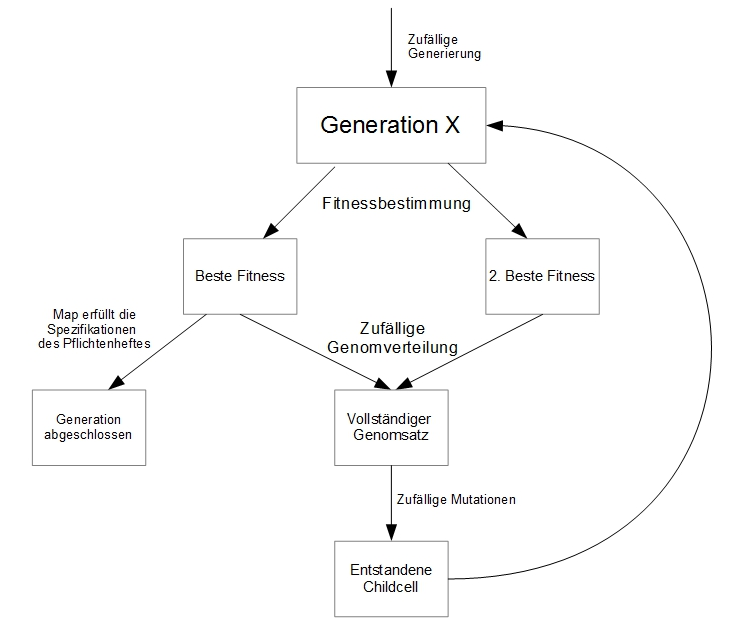
\includegraphics[width=0.8\textwidth]{Gen_Alg.png}
\end{figure}

\subsubsection{vec}
\verb+vec+ enthält Funktionen für zweidimensionale Vektormathematik.